\documentclass[paper=a4, fontsize=11pt]{scrartcl} % A4 paper and 11pt font size

\usepackage[T1]{fontenc} % Use 8-bit encoding that has 256 glyphs
\usepackage{fourier} % Use the Adobe Utopia font for the document - comment this line to return to the LaTeX default
\usepackage[english]{babel} % English language/hyphenation
\usepackage{amsmath,amsfonts,amsthm} % Math packages
\usepackage{lipsum} % Used for inserting dummy 'Lorem ipsum' text into the template
\usepackage{graphicx}
\usepackage{sectsty} % Allows customizing section commands
\allsectionsfont{\centering \normalfont\scshape} % Make all sections centered, the default font and small caps
\usepackage[utf8]{inputenc} 
\usepackage{fancyhdr} % Custom headers and footers
\pagestyle{fancyplain} % Makes all pages in the document conform to the custom headers and footers
\fancyhead{} % No page header - if you want one, create it in the same way as the footers below
\fancyfoot[L]{} % Empty left footer
\fancyfoot[C]{} % Empty center footer
\fancyfoot[R]{\thepage} % Page numbering for right footer
\renewcommand{\headrulewidth}{0pt} % Remove header underlines
\renewcommand{\footrulewidth}{0pt} % Remove footer underlines
\setlength{\headheight}{13.6pt} % Customize the height of the header

\numberwithin{equation}{section} % Number equations within sections (i.e. 1.1, 1.2, 2.1, 2.2 instead of 1, 2, 3, 4)
\numberwithin{figure}{section} % Number figures within sections (i.e. 1.1, 1.2, 2.1, 2.2 instead of 1, 2, 3, 4)
\numberwithin{table}{section} % Number tables within sections (i.e. 1.1, 1.2, 2.1, 2.2 instead of 1, 2, 3, 4)

\setlength\parindent{0pt} % Removes all indentation from paragraphs - comment this line for an assignment with lots of text

%----------------------------------------------------------------------------------------
%	TITLE SECTION
%----------------------------------------------------------------------------------------

\newcommand{\horrule}[1]{\rule{\linewidth}{#1}} % Create horizontal rule command with 1 argument of height

\title{	
\normalfont \normalsize 
\textsc{Københavns Universitet, Datalogisk Institut} \\ [25pt] % Your university, school and/or department name(s)
\horrule{0.5pt} \\[0.4cm] % Thin top horizontal rule
\huge Ugeopgave 14 - Gruppeopgave \\ % The assignment title
\horrule{2pt} \\[0.5cm] % Thick bottom horizontal rule
}

\author{Allan Nielsen, Troels Thomsen, Troels Kamp Leskes} % Your name

\date{\normalsize\today} % Today's date or a custom date

\begin{document}

\maketitle % Print the title

\section*{Design}

Vi har følgende klasser:

\begin{itemize}
	\item Vector\\
		Vector klassen beskriver en todimensionel vektor, og indeholder hjælpemetoder til skalering, prikprodukt etc.
		Vi valgte at lave vores egen klasse frem for at bruge numpy.matrix, fordi vi mente at det på denne måde var nemmere til denne begrænsede simulation når vi alligevel selv skal implementere funktioner til vektorberegning.
	\item Particle\\
		Particle klassen beskriver en enkelt partikel i vores simulation. Partiklen indeholder information omkring dens position og hastighed, samt hjælpefunktioner til hvordan den skal bevæge sig i simulationen.
		Vi valgte at lægge stepfunktionerne hos partiklen, for at undgå for tæt coupling mellem partiklerne og containeren.\\
		Vores partikle abstraktion har dog den svaghed, at den ved kollision (eller i skridtet før kollision) i visse tilfælde havner uden for beholderen. I disse tilfælde findes der ikke et u i intervallet $0 < u \leq 1$. \\
		Vi overkommer dette problem ved at vælge den absolutte værdi af u, men der findes stadig ydertilfælde hvor partiklen aldrig kan komme ind i beholderen igen.
	\item Container\\
		Container klassen beskriver vores todimentionelle cylinder med gaspartikler. Containeren genererer et givent antal partikler og tildeler dem tilfældige positioner og hastigheder. Containeren håndterer yderligere simulation af temperaturændringer.
	\item ContainerVisualiser\\
		ContainerVisualiser klassen er animerer en given simulation i tiden t, ved hjælp af matplotlib.
\end{itemize}

Vores design er centreret omkring containeren, der skaber partiklerne. Container klassen er dog "passiv" som de andre klasser, og kører rent faktisk ikke simulationen. Vores design har derfor mere form af bibliotek der kan genbruges af andre programmer, men som i sig selv ikke har nogen "main" funktion.\\

Vi har dog et par test-klasser som kører simulationen under forskellige omstændigheder og med forskellige parametre. (Se ContainerVisualiserTest)\\

\begin{figure}[h!]
  \centering
    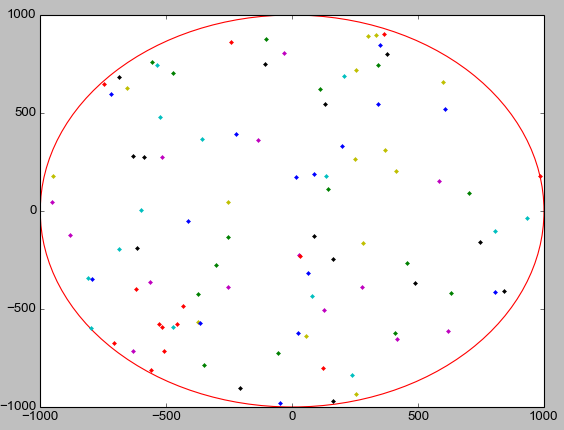
\includegraphics[width=.8\textwidth]{figure_1.png}
  \caption{Simulationen som kørt i ContainerVisualiserTest.test\_animate2()}
\end{figure}
\pagebreak


\end{document}